\section{例}

本节以4个实例介绍系统的概念,并给出其时域模型。

%============================================================
\subsection{RC电路}

\begin{example}
如下RC电路,假设电压源为系统输入信号$x\left( t \right) $,电容两端电压看作系统输出信号$y\left( t \right) $,试写出输入输出的微分方程。
\end{example}

\begin{figure}[h]
\centering
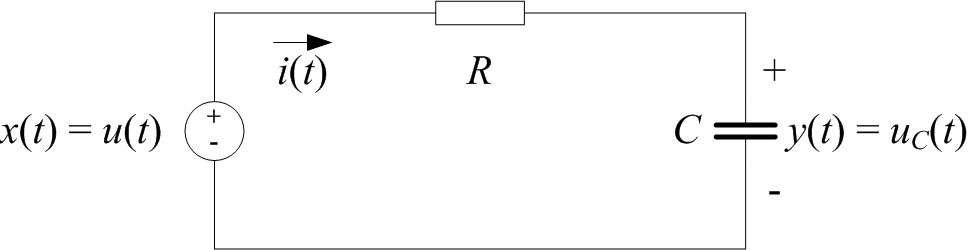
\includegraphics[height=2cm]{1.5.1-1.png}
\end{figure}

根据KVL推导RC电路的输入输出模型:
\begin{align*}
&\because u_C+u_R=u \\
&\therefore y+C\frac{dy}{dt}\cdot R=x \\
&\therefore \frac{dy}{dt}+\frac{1}{RC}y=\frac{1}{RC}x
\end{align*}
只要确定了输入信号$x=u\left( t \right) $,就可通过求解微分方程得到输出信号$y=u_C\left( t \right) $。

\begin{tcolorbox}
该RC电路会在之后的章节中反复讨论。
\end{tcolorbox}

%============================================================
\subsection{汽车运行}

\begin{example}
假设车辆在不光滑路面沿直线行驶,整个车辆作为系统,将发动机的动力视为系统输入$x$,行驶距离视为输出$y$,试写出系统的输入输出的微分方程。
\end{example}

根据牛顿定律我们可以得到车辆的加速度和受力的关系式:
\[
F=Ma
\]
车辆受力除了发动机的输出力之外,还有地面的摩擦力,摩擦力和速度成正比$K$,反向于速度方向,于是:
\[
x-K\frac{dy}{dt}=M\frac{d^2y}{dt^2}
\]
该微分方程即为车辆系统的微分方程。

%============================================================
\subsection{弹簧减震系统}

\begin{example}
如下图,系统由压块(质量$M$)、弹簧(胡克系数$K$)和阻尼器(阻尼系数$D$)组成,将压块受到的外力视为输入$x=F\left( t \right) $,压块位移视为输出$y=S\left( t \right) $,试写出输入输出的微分方程。
\end{example}

\begin{figure}[h]
\centering
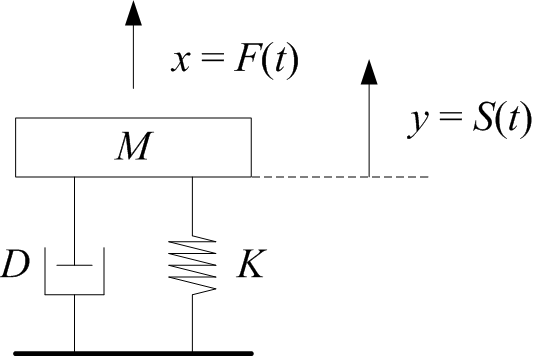
\includegraphics[height=3cm]{1.5.3-1.png}
\end{figure}

依然根据牛顿定律,考察压块的加速度和受力,弹簧施加反向作用力(大小和压块位移成正比),阻尼器施加反向作用力(大小和压块速度成正比),有:
\[
x-D\frac{dy}{dt}-Ky=M\frac{d^2y}{dt^2}
\]

%============================================================
\subsection{钟摆}

\begin{example}
假设有钟摆,输入为小球受的切向于运动方向的力$x=F\left( t \right) $,输出为偏转角$y=\theta \left( t \right) $,试写出输入输出的微分方程。
\end{example}

\begin{figure}[h]
\centering
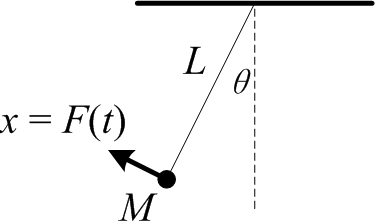
\includegraphics[height=2cm]{1.5.4-1.png}
\end{figure}

小球转动惯量为$I=ML^2$,收到两个外力$x=F\left( t \right) $和重力,它们产生的力矩分别为$xL,MgL\sin y$,根据牛顿定律对转动角加速度和力矩的关系,有:
\[
ML^2\cdot \frac{d^2y}{dt^2}=xL-MgL\sin y
\]
根据这个输入输出模型的描述,系统不是一个线性系统,无法得到解析解。
但是如果考虑偏转角很小$\sin \theta =\theta $有:
\[
ML\cdot \frac{d^2y}{dt^2}=x-Mg\cdot y
\]
变成了线性系统。
通过这样的处理后的系统称为{\bf 小信号系统}(small-signal system)。

\begin{tcolorbox}
有的时候,严格来讲,碰到的系统并不是LTI。
但是考虑到输入输出信号很小的情况下,可以近似用线性模型描述,这样的模型称为该系统的小信号模型。
在一定程度下,可以用一个简单的微分方程代替一个复杂的微分方程来考察系统。
\end{tcolorbox}




